\begin{figure}[h]
    \centering
    \begin{subfigure}[b]{0.23\textwidth}
        \centering
        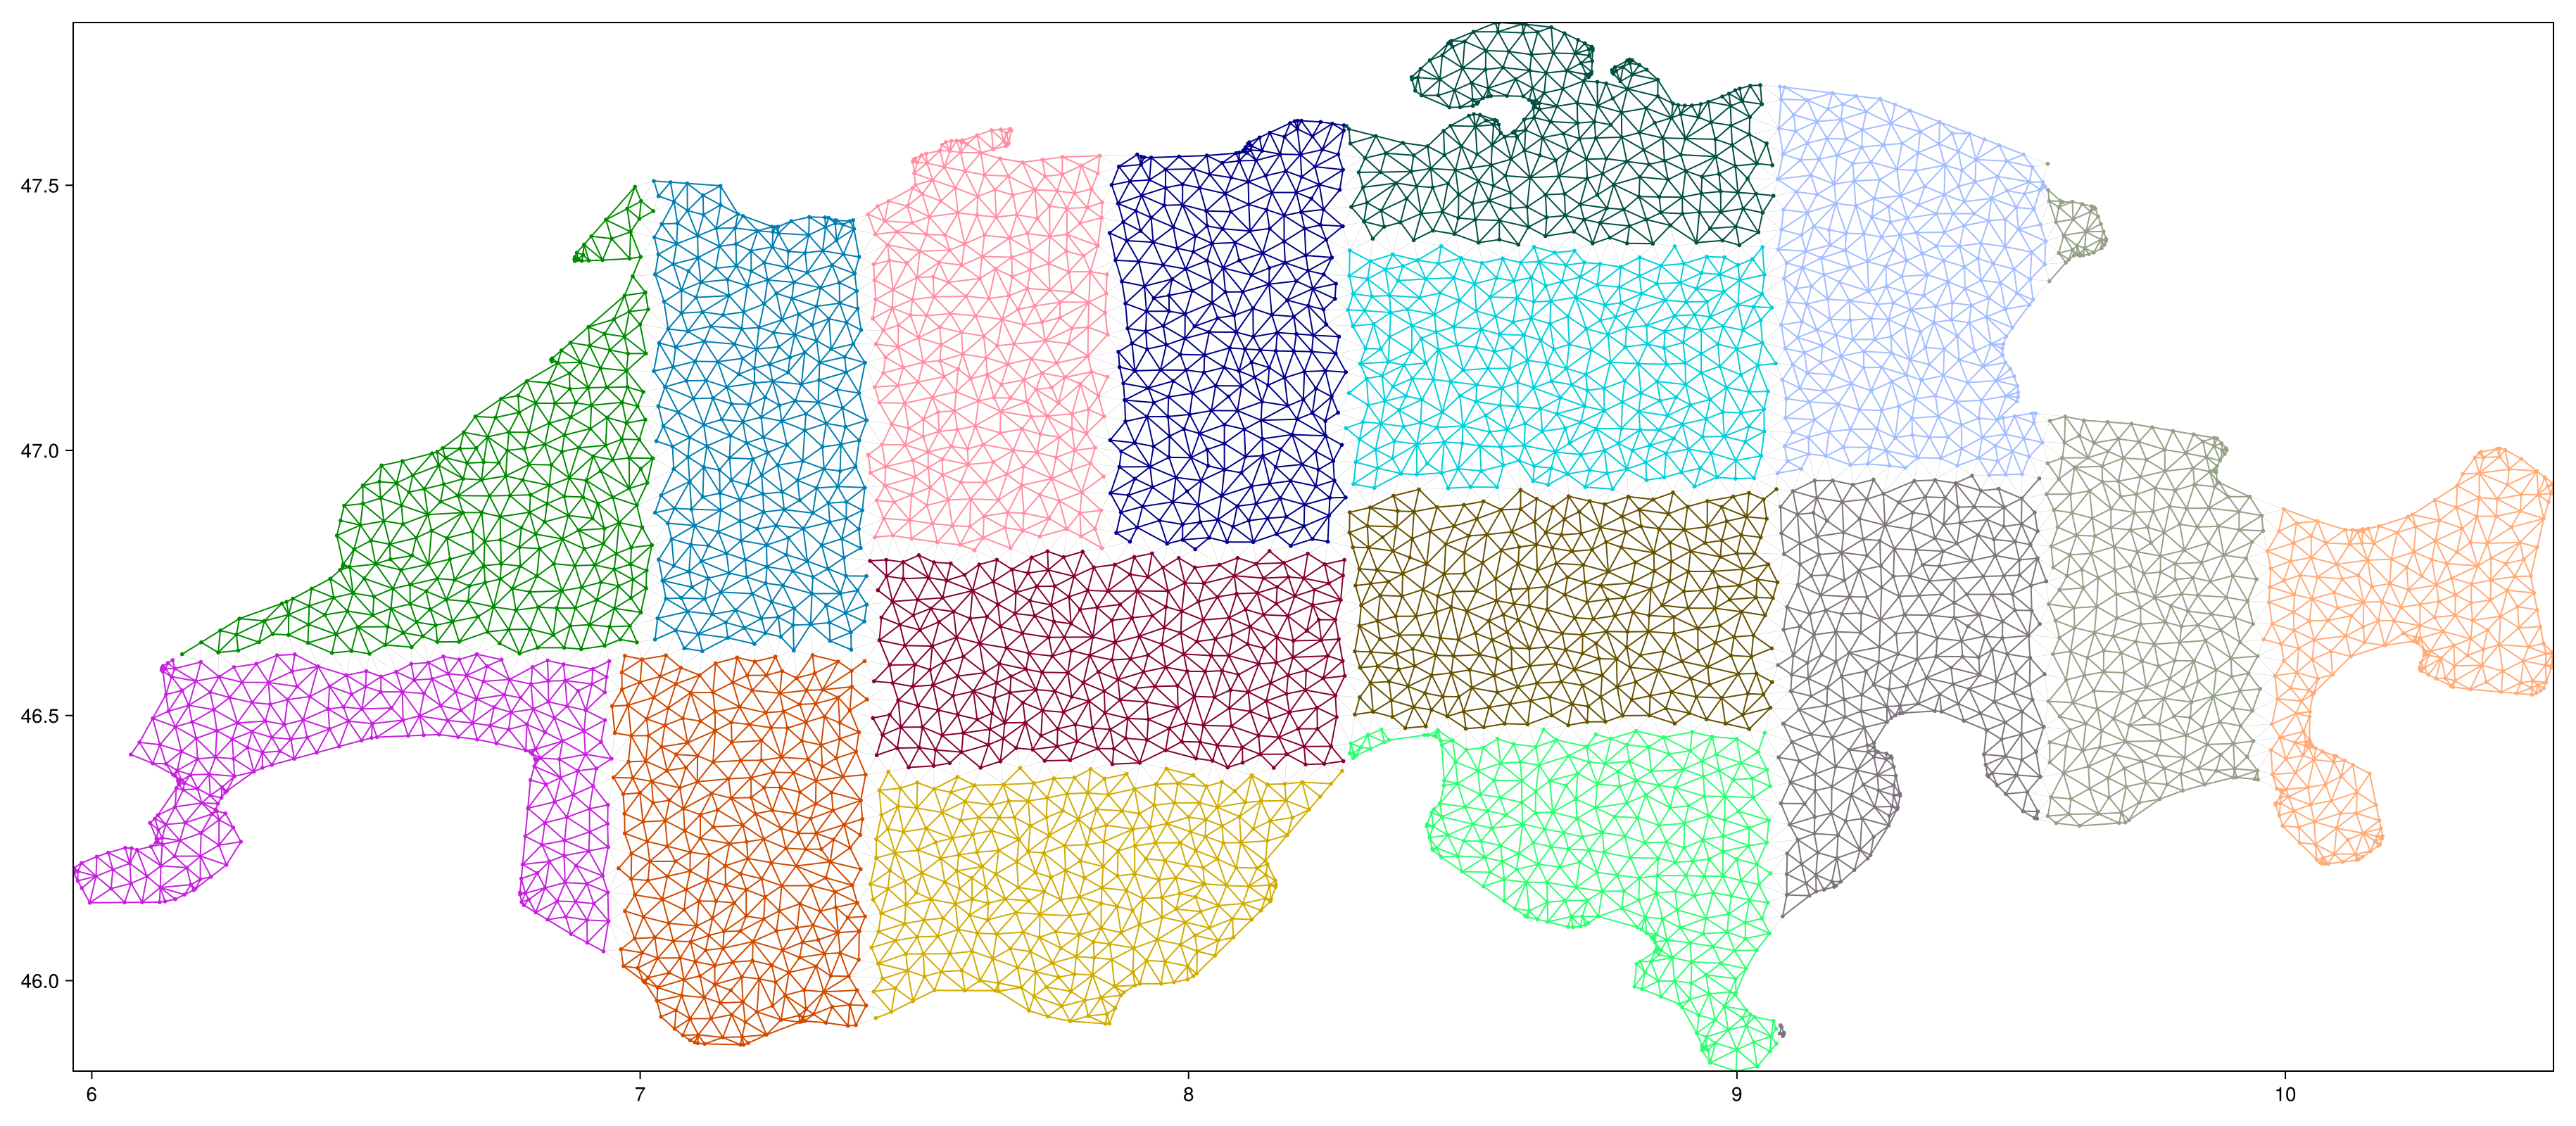
\includegraphics[width=\textwidth,  trim={98pt 70pt 0 0}, clip]{images/ex2_Swiss_graph_coordinate.png}
        \caption{Recursive coordinate bisection}
        \label{fig:ex2_coord}
    \end{subfigure}
    \hfill
    \begin{subfigure}[b]{0.23\textwidth}
        \centering
        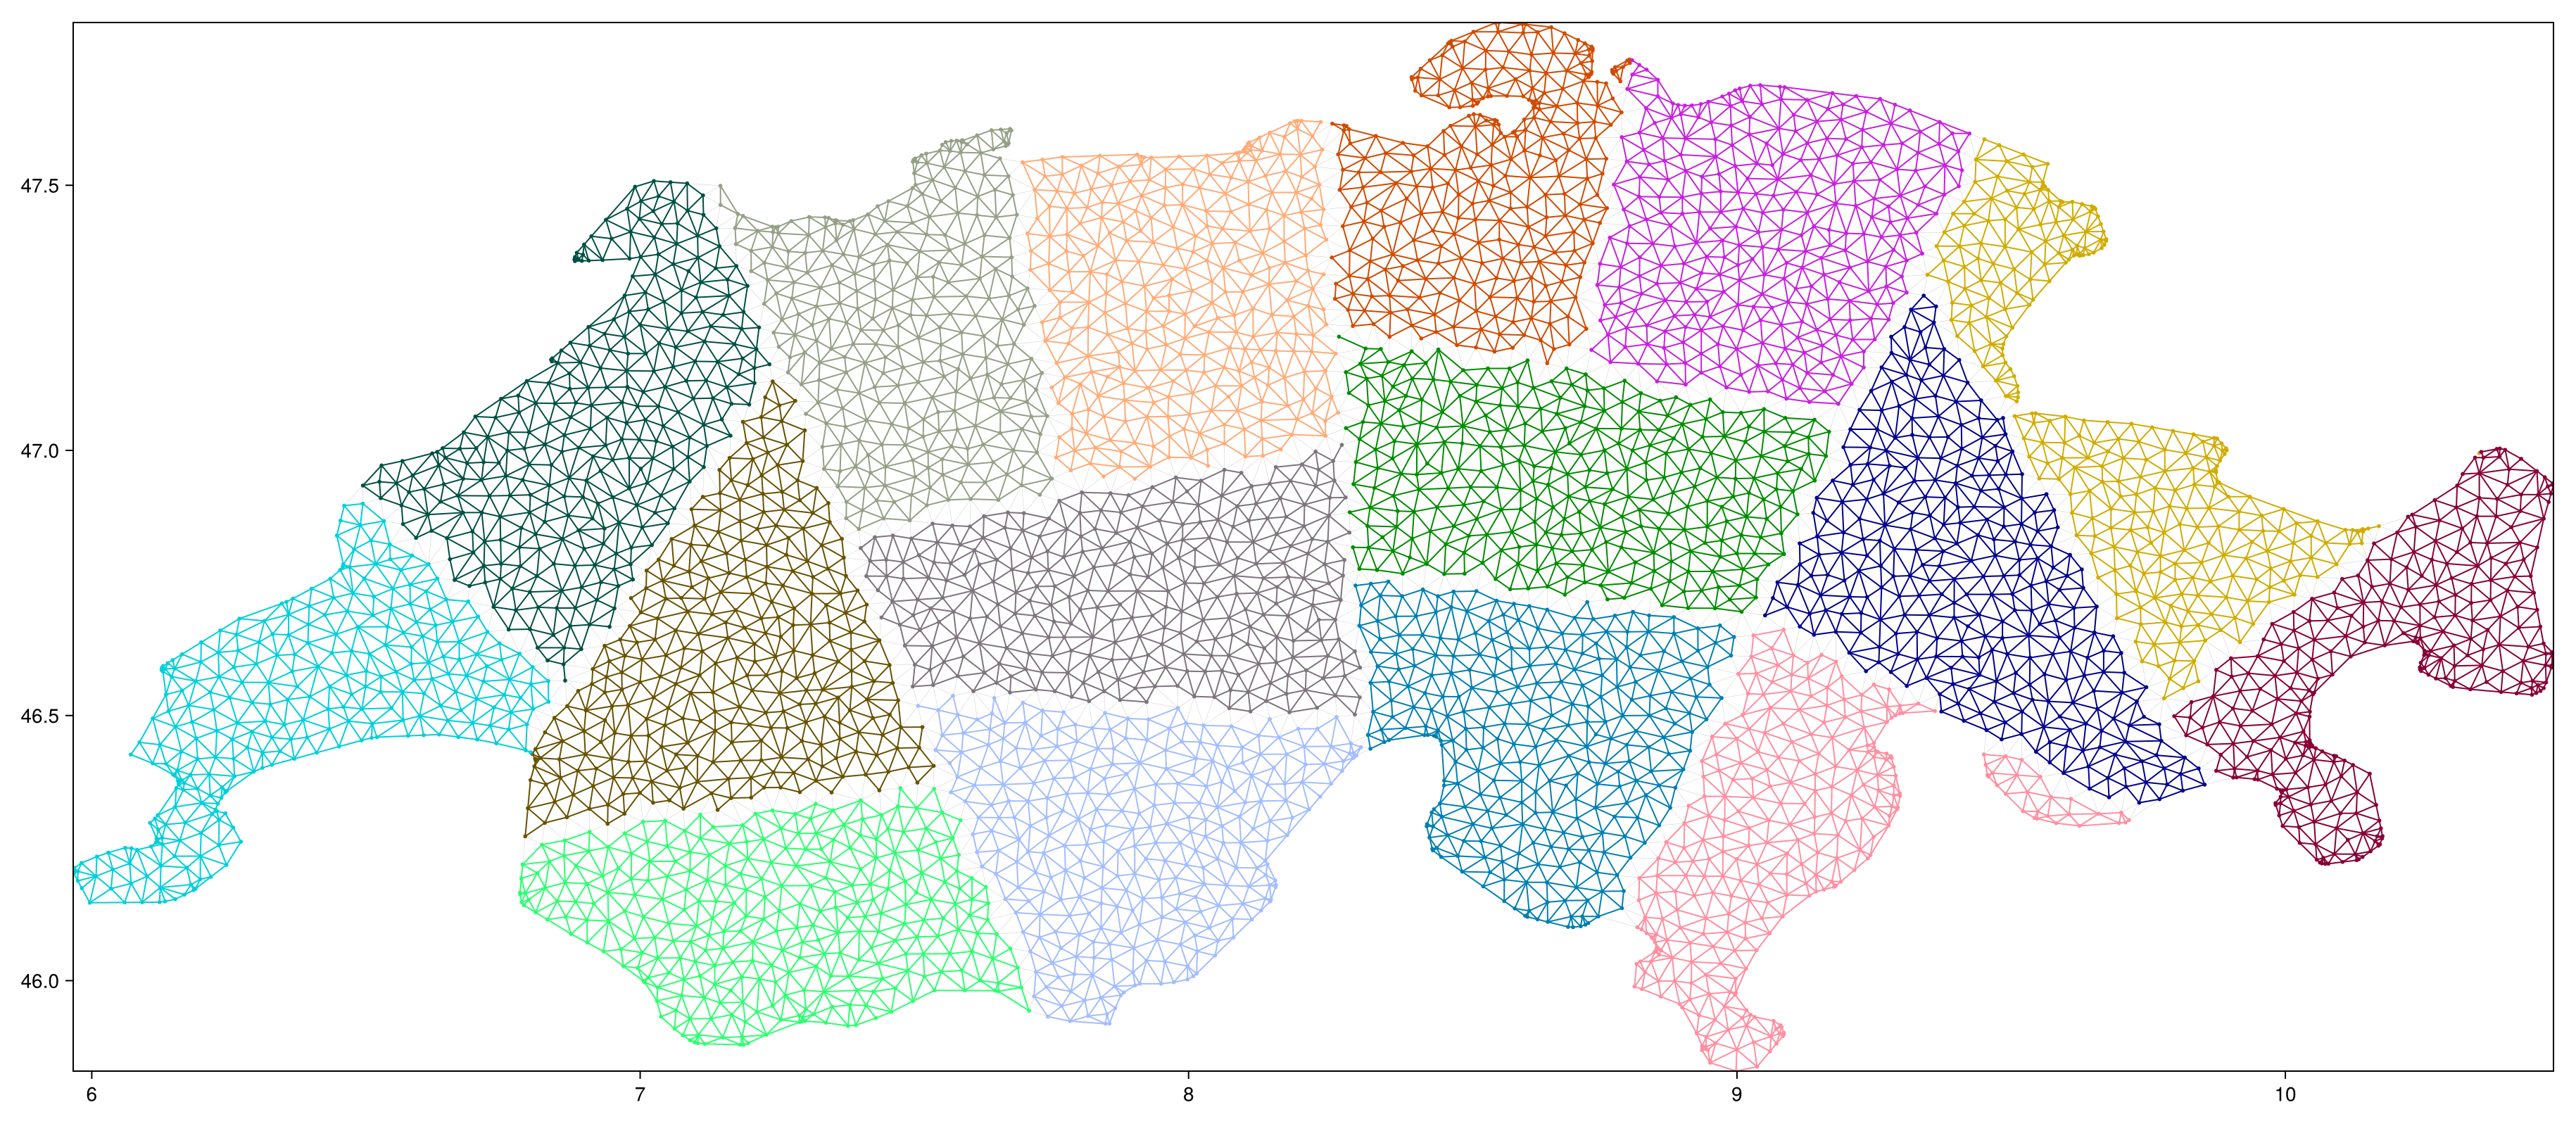
\includegraphics[width=\textwidth,  trim={98pt 70pt 0 0}, clip]{images/ex2_Swiss_graph_inertial.png}
        \caption{Recursive inertial bisection}
        \label{fig:ex2_inertial}
    \end{subfigure}

    \vskip\baselineskip  % Adds vertical space between the rows

    \begin{subfigure}[b]{0.23\textwidth}
        \centering
        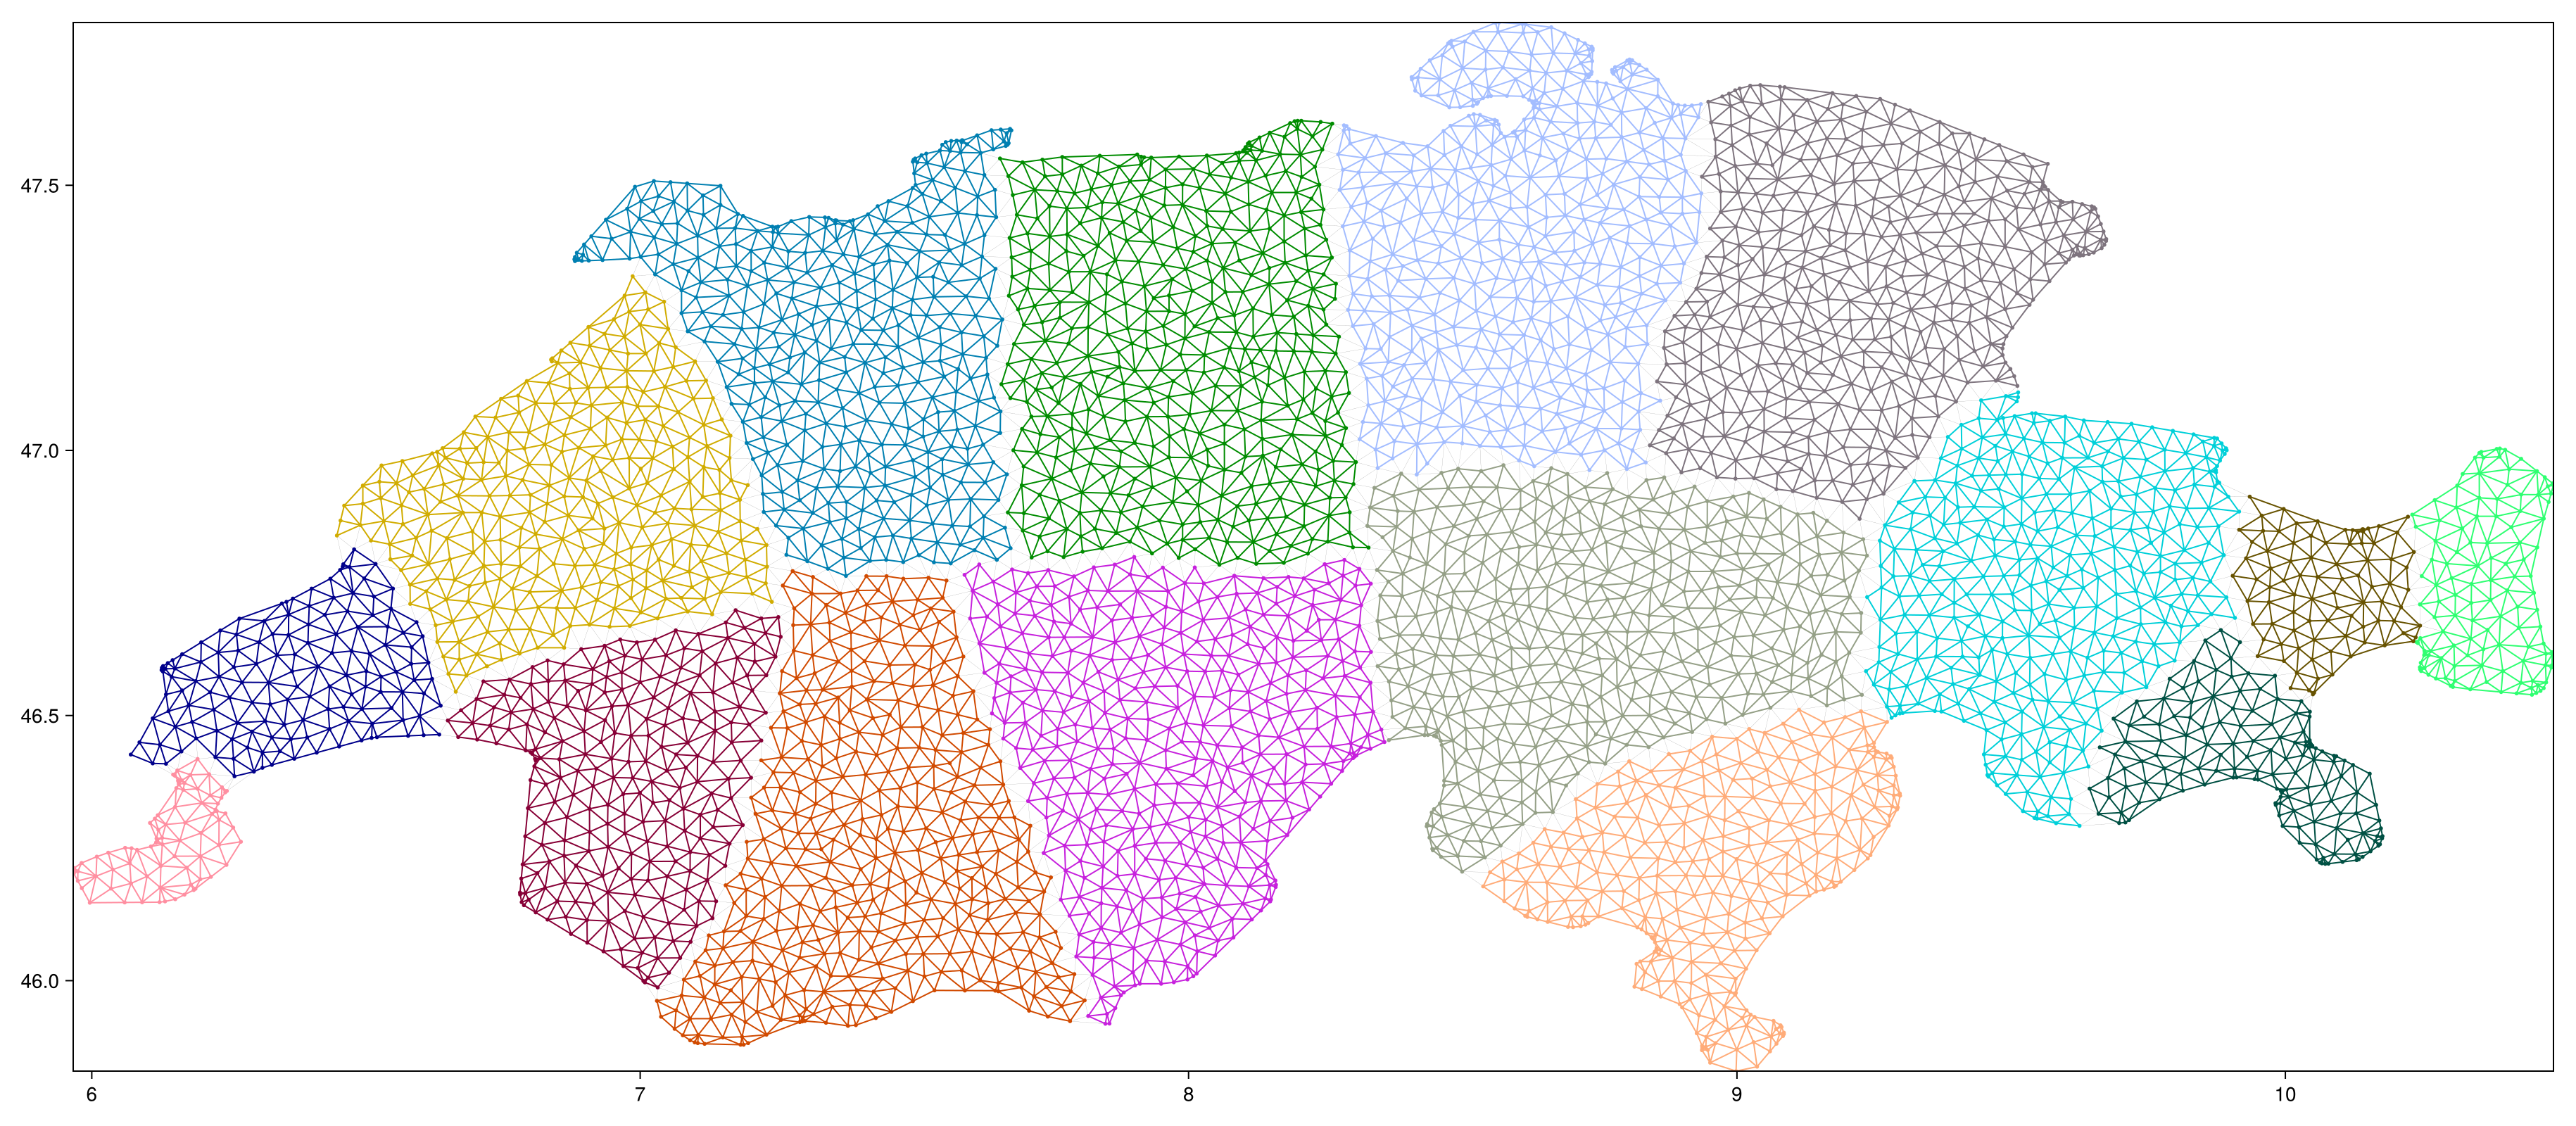
\includegraphics[width=\textwidth,  trim={98pt 70pt 0 0}, clip]{images/ex2_Swiss_graph_spectral.png}
        \caption{Recursive spectral bisection}
        \label{fig:ex2_spectral}
    \end{subfigure}
    \hfill
    \begin{subfigure}[b]{0.23\textwidth}
        \centering
        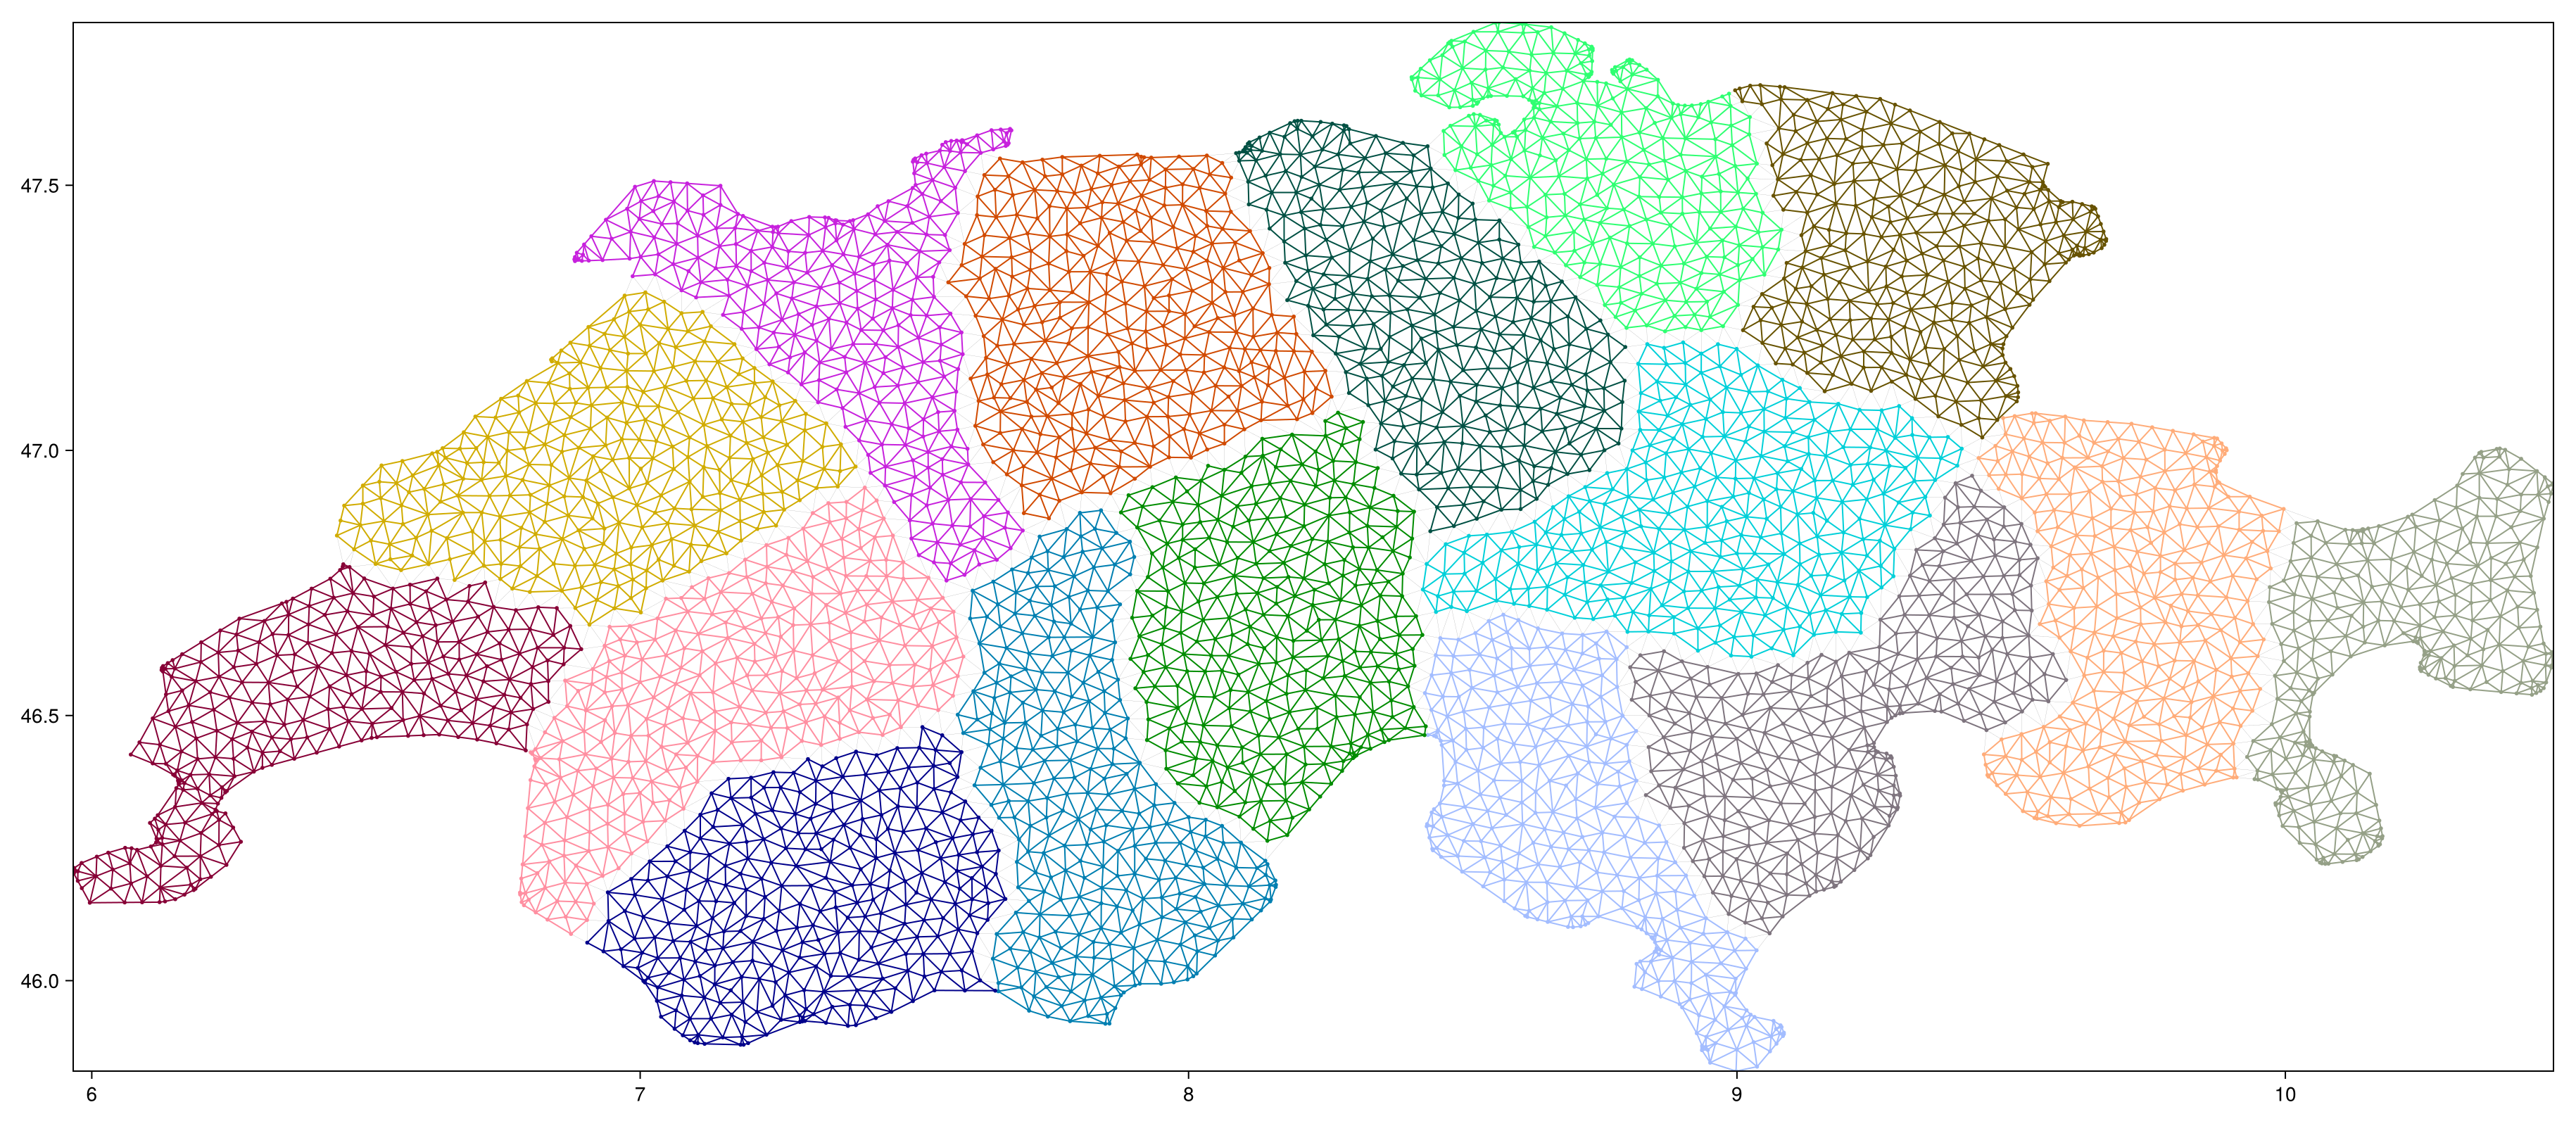
\includegraphics[width=\textwidth,  trim={98pt 70pt 0 0}, clip]{images/ex2_Swiss_graph_metis_rec.png}
        \caption{Recursive \texttt{METIS} bisection}
        \label{fig:ex2_metis}
    \end{subfigure}

    \caption{Comparison of four graph recursive bisection methods applied to the \texttt{Swiss\_graph} (4468 nodes and 15230 edges), illustrating differences in recursive partitioning results.}
    \label{fig:ex2_results}
\end{figure}


% \begin{figure}
%     \centering

%     \begin{subfigure}[b]{0.45\textwidth}
%         \centering
%         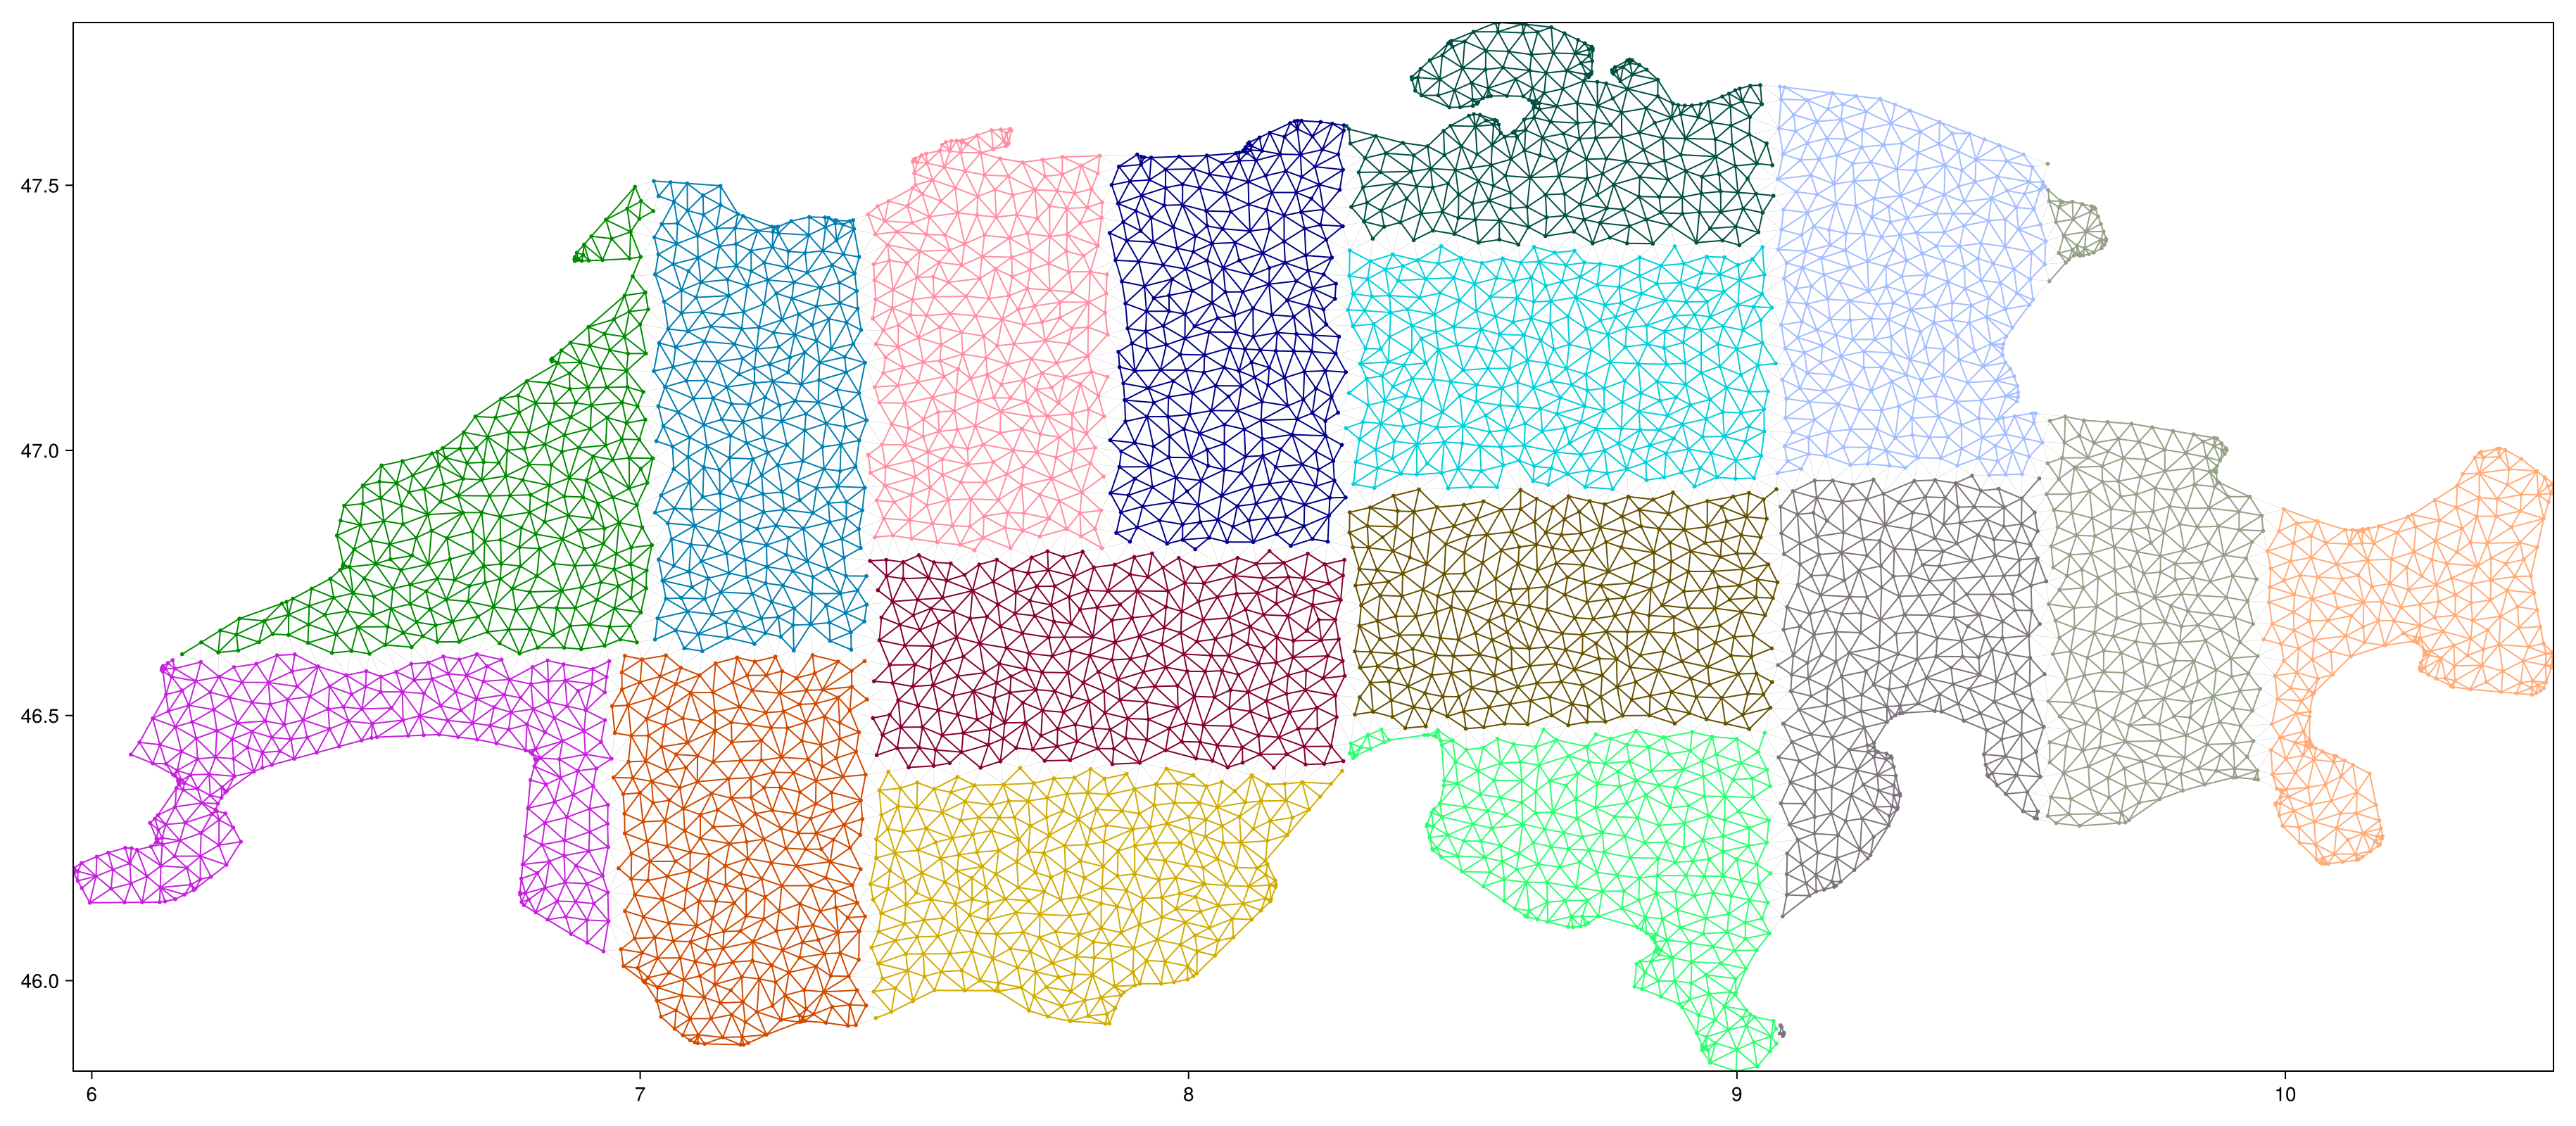
\includegraphics[width=\textwidth, trim={98pt 70pt 0 0}, clip]{images/ex2_Swiss_graph_coordinate.png}
%         \caption{Recursive coordinate bisection}
%         \label{fig:ex2_coord}
%     \end{subfigure}

%     \vskip\baselineskip

%     \begin{subfigure}[b]{0.45\textwidth}
%         \centering
%         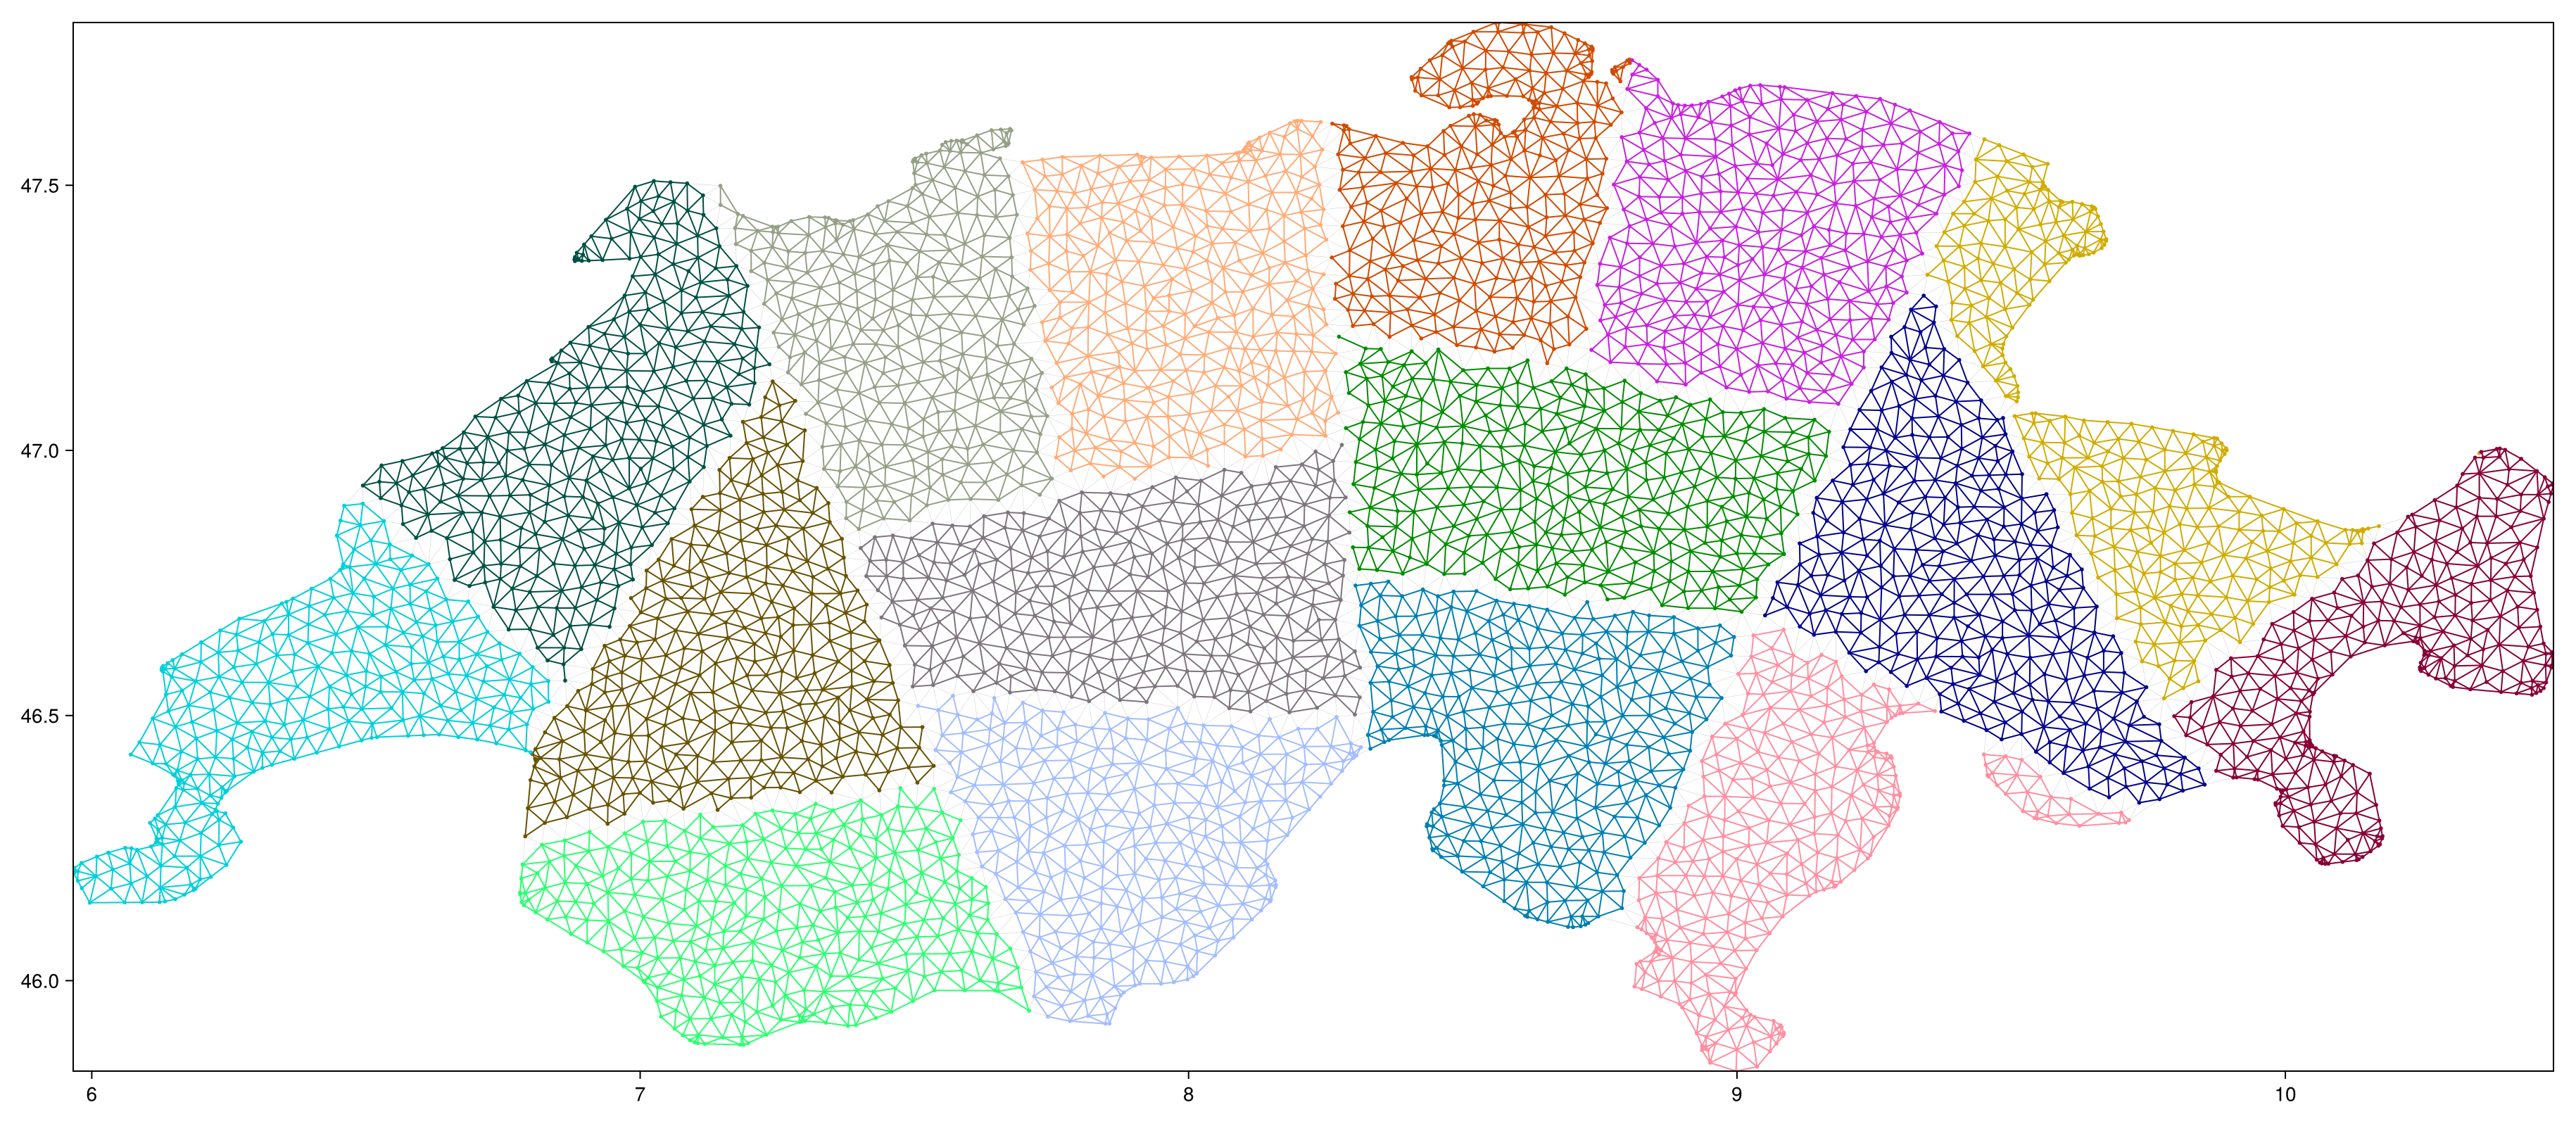
\includegraphics[width=\textwidth, trim={98pt 70pt 0 0}, clip]{images/ex2_Swiss_graph_inertial.png}
%         \caption{Recursive inertial bisection}
%         \label{fig:ex2_inertial}
%     \end{subfigure}

%     \vskip\baselineskip

%     \begin{subfigure}[b]{0.45\textwidth}
%         \centering
%         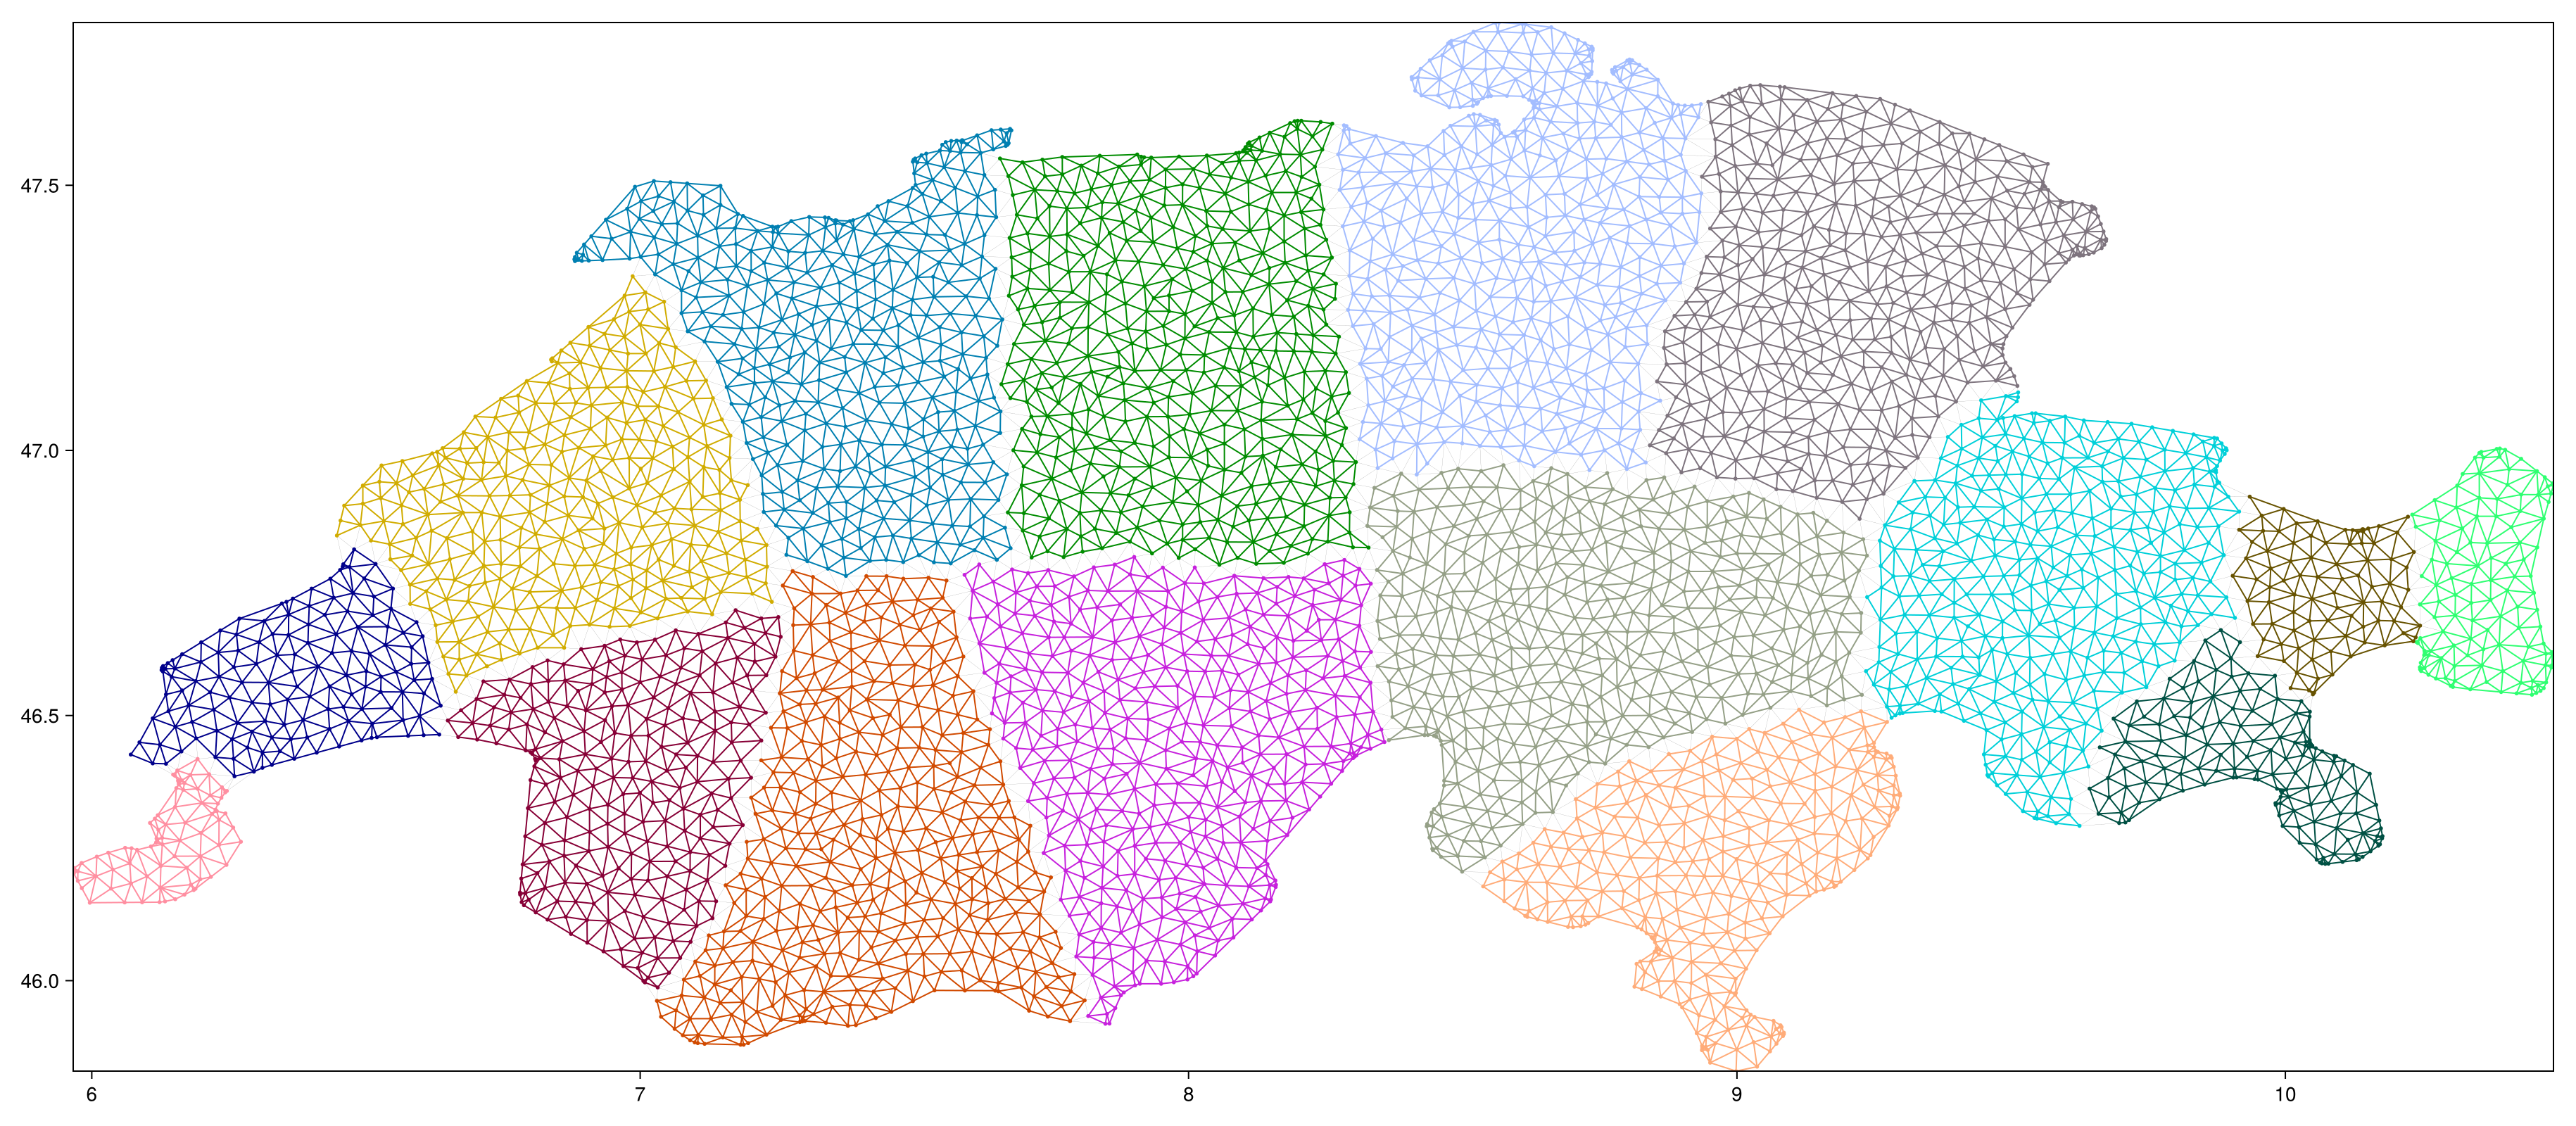
\includegraphics[width=\textwidth, trim={98pt 70pt 0 0}, clip]{images/ex2_Swiss_graph_spectral.png}
%         \caption{Recursive spectral bisection}
%         \label{fig:ex2_spectral}
%     \end{subfigure}

%     \vskip\baselineskip

%     \begin{subfigure}[b]{0.45\textwidth}
%         \centering
%         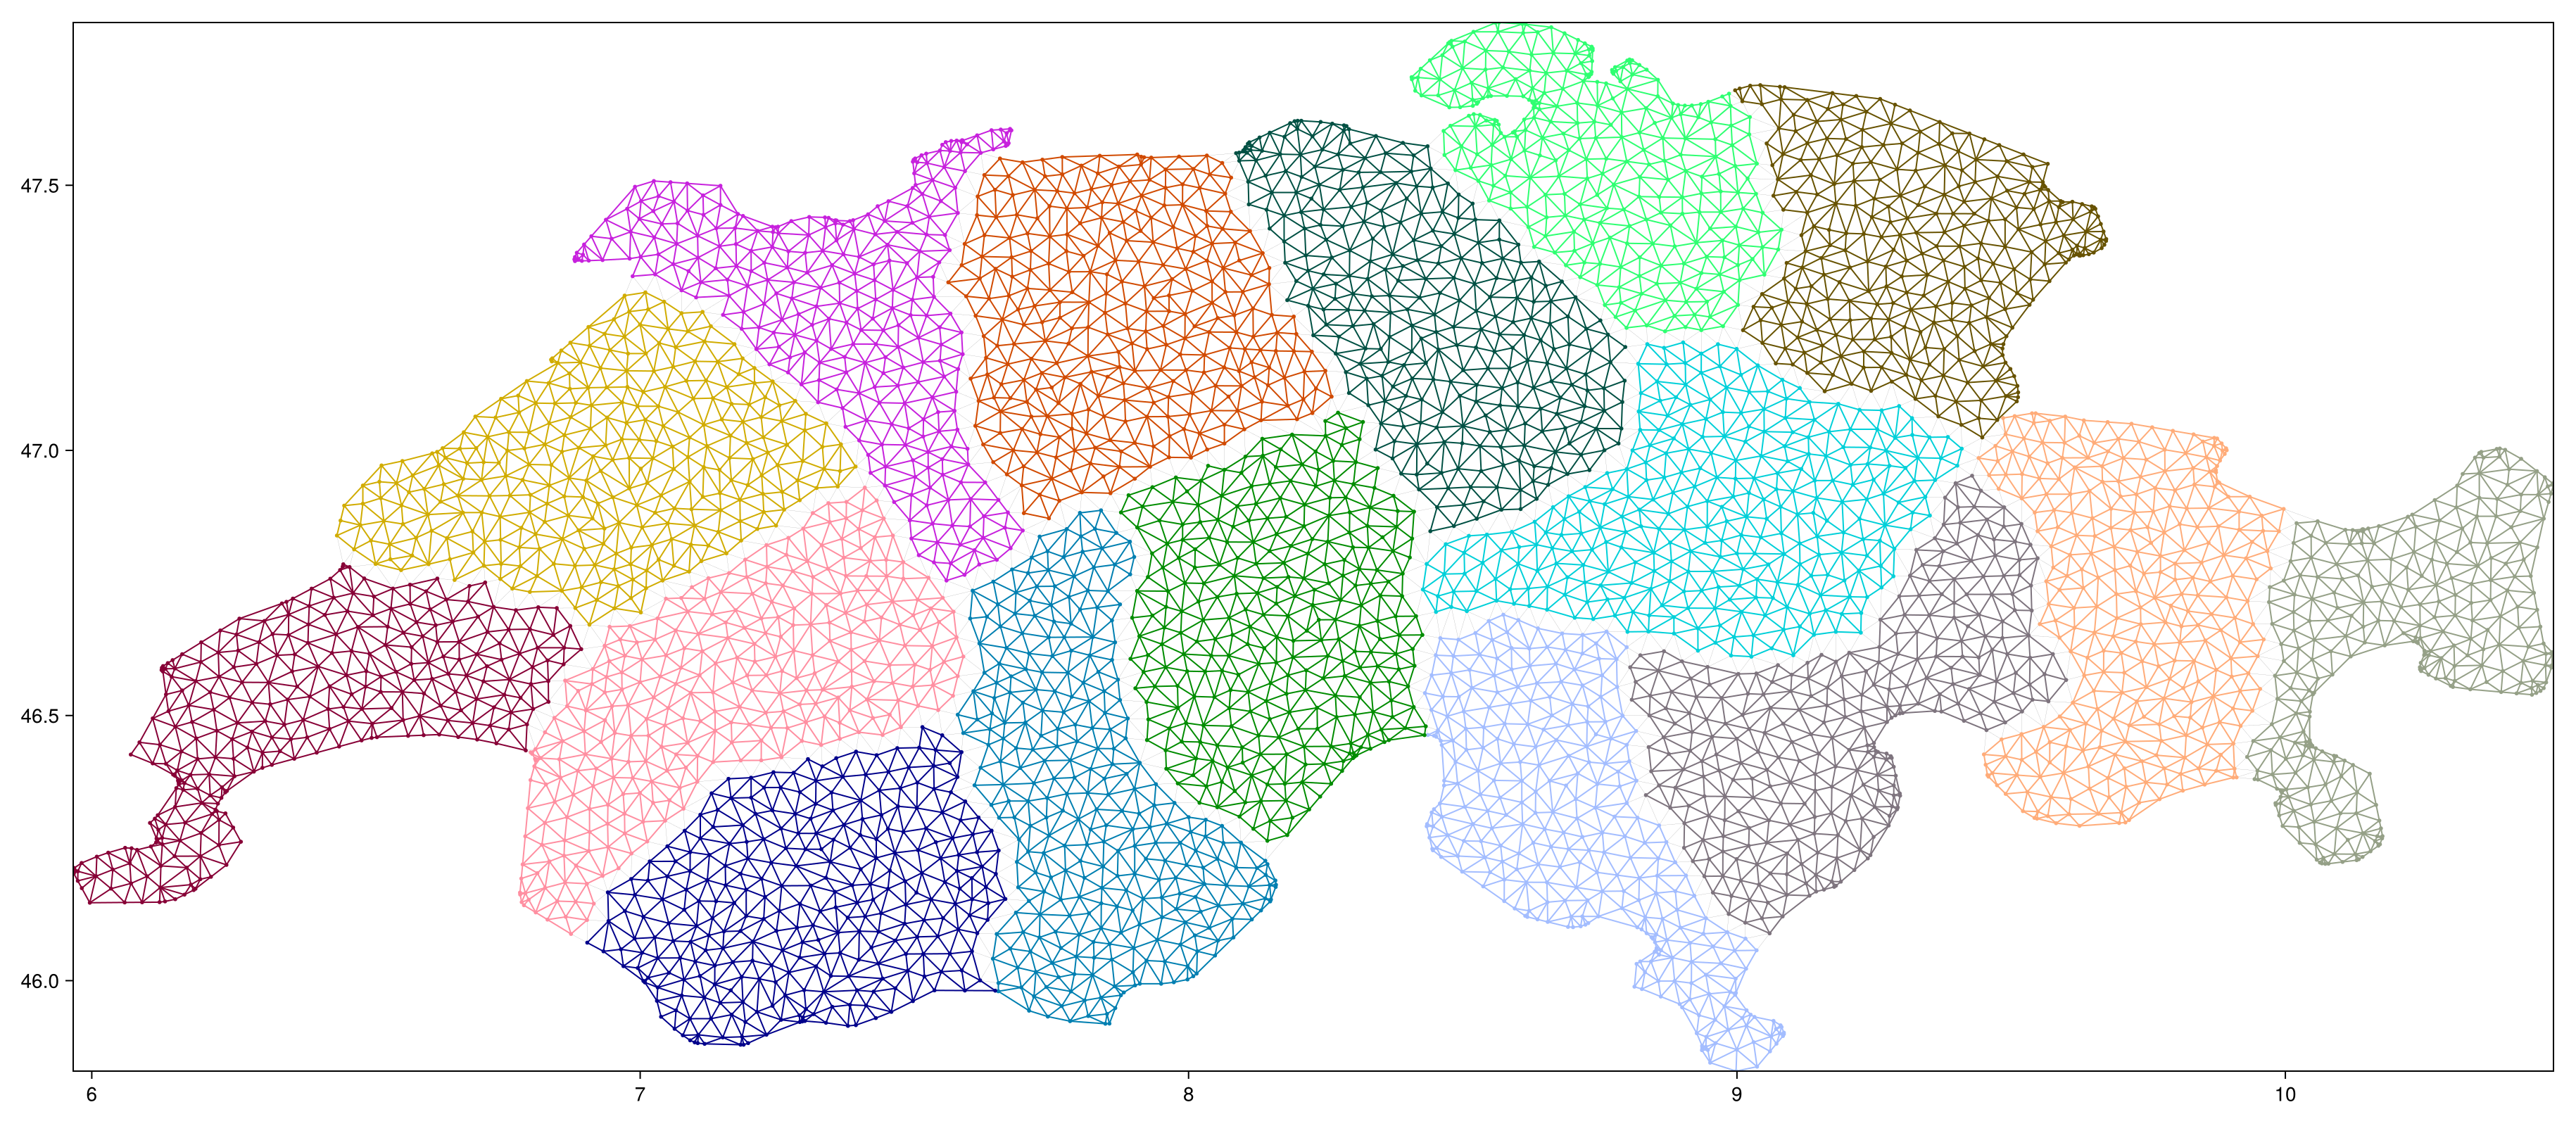
\includegraphics[width=\textwidth, trim={98pt 70pt 0 0}, clip]{images/ex2_Swiss_graph_metis_rec.png}
%         \caption{Recursive spectral bisection}
%         \label{fig:ex2_metis}
%     \end{subfigure}

%     \caption{Recursive bisection of the \texttt{Swiss\_graph} mesh using different methods. Each partition result shows the division into $p = 16$ subdomains.}
%     \label{fig:ex2_results}
% \end{figure}